%!TEX root = mieic-en.tex

\chapter{Implementation}\label{chap:chap4}
\listoftodos
\section*{}

\textit{
Este capítulo pode ser dedicado à apresentação de detalhes de nível
mais baixo relacionados com o enquadramento e implementação das
soluções preconizadas no capítulo anterior.
Note-se no entanto que detalhes desnecessários à compreensão do
trabalho devem ser remetidos para anexos.
Dependendo do volume, a avaliação do trabalho pode ser incluída neste
capítulo ou pode constituir um capítulo separado.
}


As previously stated, the work done for this project consists of a module for the "Video Server" being developed by LIACC, that will perform all the required analytics of the video received. This chapter provides the details of the implementation of this module, developed during the dissertation semester between February and June 2017. Tasks performed involved designing an appropriate architecture, able to scale with the project, treating the images received from the video streams to detect events and extract information. 

It is expected that this chapter provides some insight on how the theoretical backgrounds presented before were used during the project development, namely phase 2 and 3 of the presented project planning\missingfigure{Project Planning}. Phase 2 focused on the detection of relevant events to the traffic controller such as suspicious approximation to the camera, intrusion in prohibited areas, fallen objects on the road and wrong way travelling, while phase 3 aimed to count and classify vehicles in both urban and high-way scenarios.

\section{Technology}

In order to build this project we needed both a library of already implemented computer vision algorithms as well as a simple way to retrieve frames from both video streams and files. This section describes what were the chosen technologies including a brief description and why it was chosen.

\subsection{OpenCV}
OpenCV is a library composed of implementations of useful computer vision algorithms implementation, widely used across the industry and academy. It has interfaces for multiple programming languages, like C++, Java and Python, but is natively written in C++ in order to take advantage of low level performance enhancements, as performance is an important factor in real time computer vision applications.

The library contains over 2500 algorithms ranging from the more basic image processing such as filtering, morphology operators and geometric transformations to more complex ones that are able to, among others, compare images, track features and camera movements and recognize faces. Along with the image processing capabilities OpenCV also ships with interfaces to stereo cameras such as Kinect that allow users to retrieve a cloud of 3D points and a depth map from the captured image. This was the chosen library as there existed already previous work at LIACC using it, which could be leveraged for this project.

\subsection{JavaCV}
JavaCV is a wrapper for OpenCV written in Java that works on top of the JavaCPP Presets, a project that provides Java interfaces for commonly used C++ libraries, such as OpenCV and FFmpeg\todo{Adicionar referencias}, the ones we are using, as well as CUDA, ARToolKitPlus and others. It provides access to all the functionalities of OpenCV inside a Java environment, and was the chosen solution as there was already experience inside LIACC working with this technology.

\subsection{FFmpeg}
FFmpeg is a framework that performs encoding, decoding, transcoding, streaming and filter operations on videos in all the well known video formats, across a large number of platforms. It is used in the "Video Server" to read streams from any format and restream them all to the same format. In the Analytic module it is used to grab the frames from both the video files and the streams using the same methods.

\begin{lstlisting}[float,language=Java, label=src:ffmpegframegrabber, caption=FFmpegFrameGrabber usage example] 

// videopath can be either a stream path or a file path
FFmpegFrameGrabber _frameGrabber = FFmpegFrameGrabber.createDefault(videopath);
Frame currentFrame = null;

while( (currentFrame = _frameGrabber.grabImage()) != null) {
	// Use grabbed frame
}

\end{lstlisting}

\section{Architecture}

\subsection{Implementation Architecture}

\missingfigure{Diagrama Arquitetura}

The analytics module was designed to comply with the following specifications, imposed by both our partner and to comply with the already developed modules. 

\begin{itemize}
	\item Run uninterruptedly waiting for requests to be made
	\item Process a large number of video inputs at the same time
	\item Receive input from streams or files
	\item Specify which analysis are to be run on a specific video
\end{itemize}
\todo{Mais requirements?}

The project main thread runs an instance of the AnalyticsManager class that implements the Java Runnable interface. This thread will launch one CameraAnalyticsManager instance for each video to be analysed, be it from stream or from file, and keep track of each worker status, disposing of them when they finish, and launching new ones when a request is received. The CameraAnalyticsManager is then responsible to query the database in order to find out what are the analytics the user wants to retrieve from the video, information that is stored in the \textit{camera} table of the database. This process then starts a frame grabber that will convert each frame of the video into its representation in OpenCV and feed it to each Analyser through a queue. This enables each one of these workers to run at his own pace and if one of them runs slower than the pace at which the frame grabber reads the images, it will simply queue them up and not slow down the remaining workers. The drawbacks of this solution are that it is theoretically possible to run out of memory to keep these frames, although this limit was not reached during the testing phase.

\subsection{Database}

\todo{Sera relevante?}
Camaras sao o principal ator

Videos (streams e ficheiros) estao associados a uma camara


\section{Segmentation}

This section describes how the segmentation of the received images is performed, and how it returns a foreground mask representing the moving areas of the scene, specifying through what processors and filters it is passed through. \todo{Overview do processo?}

\begin{figure}[t]
  \begin{center}
    \leavevmode
    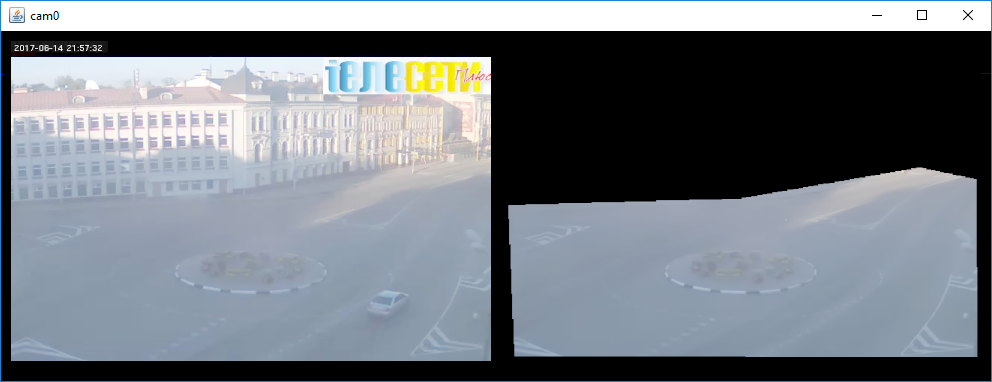
\includegraphics[width=0.95\textwidth]{bgsub_01}
    \caption{Background Subtraction - Background Model}
    \label{fig:bgsub_01}
  \end{center}
\end{figure}

In ~\ref{fig:bgsub_01} we can see the original frame on the left and the calculated background model of the scene on the right. To achieve this result, the first step is to mask the obtained frame\todo{Explain masking process} in order to prevent uninteresting regions of the image from even making it into the Background Subtracter. This solves an issue where moving or changing regions of the image outside our region of interest would create unwanted artefacts, for example moving trees due to the wind blowing, or the issue that occurred in this scene, where a car passing would be reflected in the windows of the building.

The next step of the Segmentation process is to feed the masked frames into a Background Subtraction algorithm that will use them to update its internal representation of the scene. This project uses the OpenCV implementation of the Mixture of Gaussians algorithm that allows the user to tune:

\begin{itemize}
	\item Number of past frames considered on the background calculation
	\item Threshold value from which a pixel is considered to be foreground, compared to the difference between its current value and the one from the background model
	\item Learning rate of the algorithm, how much each new frame influences the model
\end{itemize}

After updating the background model we can retrieve from the Background Subtracter its foreground mask, a rough representation that is calculated by subtracting the background model from the current image and thresholding it, thus returning only the pixels where the difference is significant enough.

\begin{figure}[t]
  \begin{center}
    \leavevmode
    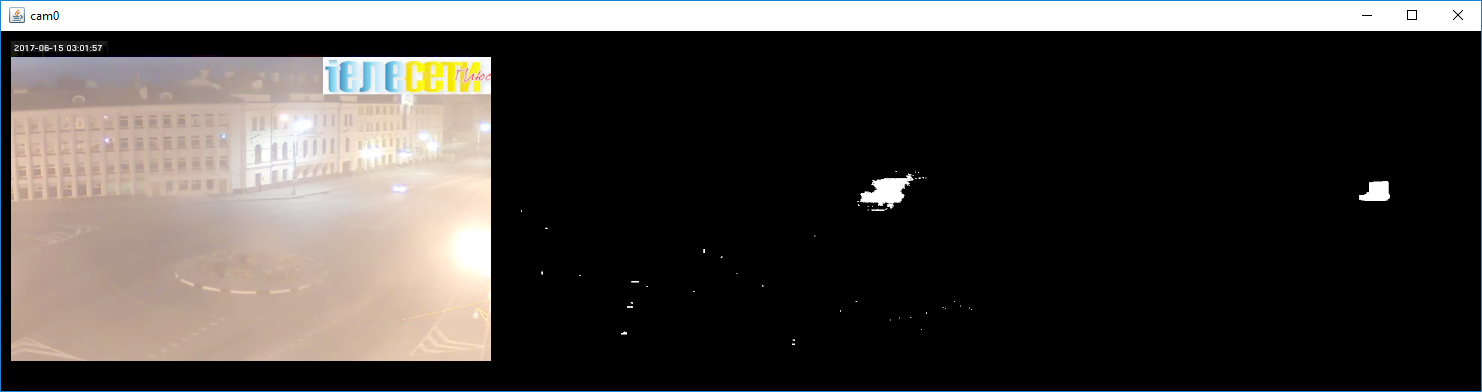
\includegraphics[width=0.95\textwidth]{bgsub_03}
    \caption{Background Subtraction - Foreground Mask}
    \label{fig:bgsub_02}
  \end{center}
\end{figure}

As we can see in the middle image of figure ~\ref{fig:bgsub_02} the foreground mask from the Background Subtracter can have a lot of noise due to lighting conditions. To solve this issue two morphology filters are applied to the image, a squared erosion filter to remove the small speckles that appear in the mask, followed by a larger circular dilation filter to consolidate the positive regions of the mask, as the wind shield and windows of the vehicles are usually detected as background due to their dark colour and/or reflection of the environment.

\section{Utility}

\subsection{Video Wall}

\subsection{Image Processors}

\section{Secção Exemplo}

%\todofigure{Inserir uma figura sobre o Map/Reduce}

Lorem ipsum dolor sit amet, consectetuer adipiscing elit. Integer
hendrerit commodo ante. Pellentesque nibh libero, aliquam at, faucibus
id, commodo a, velit. 
%\todoline{Escrever sobre o map/reduce}
Duis eleifend sem eget leo. Morbi in est. Suspendisse magna sem,
varius nec, hendrerit non, tincidunt quis, quam. Aenean congue. 
%\todolines{A short entry in the list of todos}{A very long todonote
%  that certainly will fill more than a single line in the list of
%  todos. Just to make sure let's add some more text.} 
Vivamus vel est sit amet sem iaculis posuere. Cras mollis, enim vel
gravida aliquam, libero nunc ullamcorper dui, ullamcorper sodales
lectus nulla sed urna. Morbi aliquet porta risus. 
Proin vestibulum ligula a purus. Maecenas a nulla. 
Maecenas mattis est vitae neque auctor tempus. Etiam nulla dui,
mattis vitae, porttitor sed, aliquet ut, enim. Cras nisl magna,
aliquet et, laoreet at, gravida ac, neque. Sed id est. Nulla dapibus
dolor quis ipsum rhoncus cursus.

\section{Mais uma Secção}

Lorem ipsum dolor sit amet, consectetuer adipiscing elit. Quisque
purus sapien, interdum ut, vestibulum a, accumsan ullamcorper,
erat. Mauris a magna ut leo porta imperdiet. Donec dui odio, porta in,
pretium non, semper quis, orci. Quisque erat diam, pharetra vel,
laoreet ac, hendrerit vel, enim. Donec tristique luctus risus. Fusce
dolor est, eleifend id, elementum sit amet, varius vitae, neque. Morbi
at augue. Ut sem ligula, auctor vitae, facilisis id, pharetra non,
lectus. Nulla lacus augue, aliquam eget, sollicitudin sed, hendrerit
eu, leo. Suspendisse ac tortor. Mauris at odio. Etiam vehicula. Nam
lacinia purus at nibh. Aliquam fringilla lorem ac justo. Ut nec
enim. 
%\todoref{Citar Map/reduce}

Quisque ullamcorper. Aliquam vel magna. Sed pulvinar dictum
ligula. Sed ultrices dolor ut turpis. Vivamus sagittis orci malesuada
arcu venenatis auctor. Proin vehicula pharetra urna. Aliquam egestas
nunc quis nisl. Donec ullamcorper. Nulla purus. Ut suscipit lacus
vitae dui. Mauris semper. Ut eget sem. Integer orci. Nam vitae dui
eget nisi placerat convallis. 

\begin{lstlisting}[float,language=Java, label=src:mapreduce, caption=Example map and reduce functions for word counting]
map(String key, String value): 
// key: document name 
// value: document contents 
for each word w in value:
EmitIntermediate(w, "1");

reduce(String key, Iterator values):
// key: a word 
// values: a list of counts 
int result = 0;
for each v in values: 
result += ParseInt(v);

Emit(AsString(result))
\end{lstlisting}

Sed id lorem. Proin gravida bibendum lacus. Sed molestie, urna quis
euismod laoreet, diam dolor dictum diam, vitae consectetuer leo ipsum
id ante. Integer eu lectus non mauris pharetra viverra. In feugiat
libero ut massa. Morbi cursus, lorem sollicitudin blandit semper,
felis magna pellentesque lacus, ut rhoncus leo neque at tellus. Sed
mattis, diam eget eleifend tincidunt, ligula eros tincidunt diam,
vitae auctor turpis est vel nunc. In eu magna. Donec dolor metus,
egestas sit amet, ultrices in, faucibus sed, lectus. Etiam est enim,
vehicula pharetra, porta non, viverra vel, nunc. Ut non sem. Etiam nec
neque. 

\section{Resumo ou Conclusões}

Proin vehicula pharetra urna. Aliquam egestas
nunc quis nisl. Donec ullamcorper. Nulla purus. Ut suscipit lacus
vitae dui. Mauris semper. Ut eget sem. Integer orci. Nam vitae dui
eget nisi placerat convallis. 
